\documentclass{article}
\usepackage[utf8]{inputenc}
\usepackage[ngerman]{babel}
\usepackage{amsmath}
\usepackage{amsfonts}
\usepackage{listings}
\usepackage{xcolor}
\usepackage{hyperref}
\usepackage{graphicx}

\newtheorem{definition}{Definition}

\definecolor{codegreen}{rgb}{0,0.6,0}
\definecolor{codegray}{rgb}{0.5,0.5,0.5}
\definecolor{codepurple}{rgb}{0.58,0,0.82}
\definecolor{backcolour}{rgb}{0.95,0.95,0.92}

\lstdefinestyle{mystyle}{
    language=Java,
    backgroundcolor=\color{backcolour},   
    commentstyle=\color{codegreen},
    keywordstyle=\color{magenta},
    numberstyle=\tiny\color{codegray},
    stringstyle=\color{codepurple},
    basicstyle=\ttfamily\footnotesize,
    breakatwhitespace=false,         
    breaklines=true,                 
    captionpos=b,                    
    keepspaces=true,                 
    numbers=left,                    
    numbersep=5pt,                  
    showspaces=false,                
    showstringspaces=false,
    showtabs=false,                  
    tabsize=2
}

\lstset{style=mystyle}


\title{Vergleich und Implementierung zweier Algorithmen zum Berechnen der Heaviest Increasing Sequence}
\author{Leonardowitsch Auterhoff }
\date{August 2022}

\begin{document}
\newcommand{\an}{$a_1a_2a_3$\dots$a_n$}
\maketitle

\tableofcontents

\newpage

\begin{abstract}
    In dieser Arbeit werden zwei Algorithmen zum Lösen des HIS-
    Problems vorgestellt, verglichen und implementiert. Ein dynamisch programmierter und einer aus dem Bereich der Bioinformatik. Es hat sich im Verlauf der Arbeit rausgestellt, dass beide Algorithmen in der Funktionsweise identisch sind. Es handelt sich bei dem aus der Bioinformatik um eine allgemeinere Problembeschreibung von dem ein Spezialfall das HIS-Problem löst und dessen Konkretisierung auf den dynamisch programmierten zurückführt. Deshalb ist die Implementierung nur für den dynamisch Programmierten angegeben mit einer einfach verketten Liste und einem Fenwick Tree. Es stellt sich raus, dass ein Fenwick Tree in der Laufzeit vorteilhafter gegenüber einer Liste ist, um das HIS-Problem zu lösen.
\end{abstract}


\section{Einführung}

Bei einer gegebenen Folge an Buchstaben eines geordneten Alphabets, auf welcher ein Gewicht definiert ist, ist eine \textit{Heaviest
Increasing Subsequence}(HIS) (größte, streng monotone Teilfolge) die Teilfolge, welche streng monoton ist und zudem die Summe der Gewichte der Teilfolgenglieder am Größten allen möglicher streng monotonen Teilfolgen ist. Dabei spielt die Eindeutigkeit solch einer Folge keine Rolle.\\
Eine einfachere Umschreibung wäre wie folgt:
\begin{quote}
    \small Man hat eine endliche Liste an Zahlen, die man von links nach rechts durchläuft. Dabei werden Zahlen so herausgenommen, dass jede weitere gezogene Zahl größer als die vorherige sein muss. Mit welcher Zahl man beginnt, ist nicht vorgegeben. Am Ende eines Durchganges wird die Summe aller gezogenen Zahlen ermittelt. Die Frage ist nun: Welche Karten müssen gezogen werden, sodass die Summe am Ende am größten ist?
    \end{quote}
Erste Überlegungen zum Lösen dieses Problems haben sich aus dem verwandten Problem der \textit{Longest Increasing Subsequence}(LIS) (längste, streng monotone Teilfolge) ergeben. Dabei handelt es sich um einen DP Algorithmus, d.h. es wird eine Tabelle mit einer festen, aber abhängigen Größe initialisiert und dann Eintrag für Eintrag nacheinander gefüllt. Dabei dürfen nur Werte aus der gegebenen Folge oder schon eingetragene Tabellenwerte für die Berechnung genutzt werden. Weiterführende Anwendungen der HIS und LIS sind in der Algebra, v.a. in den Permutationsgruppen, zu finden\cite{schensted1961longest}.\\
Der zweite Algorithmus kommt aus der Bioinformatik. Kern des Algorithmus' ist der Vergleich zweier bekannter Genome, in denen $"$ähnliche$"$ Abschnitte bekannt sind und gegenübergestellt werden, so dass keine Überlappung entsteht.

\section{Notation und Begrifflichkeiten}
In diesem Kapitel werden Notationen bezüglich Teilfolgen, Gewichtung und Sequenzierungen eingeführt. Im zweiten Teil wird dann auf Begriffe aus der Programmierung und Theoretischen Informatik eingegangen.

\subsection{Notation}
\subsubsection{(Teil-)Folgen}
Sei $(a_n)_{n\in\mathbb{N}}$ eine Folge an Buchstaben $a$ über einem Alphabet $\Sigma$ (im weiteren betrachten wir nur die natürlichen Zahlen $\mathbb{N}$ oder andere geordnete Mengen). Wir nennen $(a_n)$ endlich, falls es ein $n\in\mathbb{N}$ gibt, so dass für alle $k\leq n$ $a_k$ definiert ist, und sonst nicht. Im Folgenden werden wir endliche Folgen mit $a_1a_2a_3$\dots$a_n$ notieren. Man nennt eine Folge streng monoton steigend, wenn $a_i < a_{i+1}$ für alle $1\leq i < n$ gilt.\\
Eine Teilfolge von $(a_n)$ ist eine Folge $(b_k)$ für die es $i_1<i_2<$\dots$<i_k$ gibt, s.d.$a_{i_1}a_{i_2}a_{i_3}$\dots$a_{i_k}$ gleich $(b_k)$ entspricht. Betrachtet man $4,3,6,8,1,5$, so wäre $4,6,8$ mit $i_1=1,i_2=3,i_3=4$ eine streng monoton steigende Teilfolge.

\subsubsection{Gewichtungen}
Eine Gewichtungs-Funktion ist eine Zuordnungsfunktion $\Omega:\Sigma\rightarrow\mathbb{N}$ eines Alphabets $\Sigma$ auf die natürlichen Zahlen. Im Allgemeinen werden wir iuns n dieser Arbeit auf den Wert der Zahlen als Gewicht beziehen, die Gewichtsfunktion wäre damit die Identität $Id_\mathbb{N}:x \mapsto x$. Jedoch können auch andere Funktionen für das Gewicht hergenommen werden für die Algorithmen. Diese Gewichtung dient auch als Erweiterung für die Monotonie, statt $a_i<a_{i+1s}$, kann man auch $\Omega (a_i) < \Omega (a_{i+1})$ schreiben. 

\subsubsection{'Rechteck'}
Gegeben seien zwei Paare $s:=(a,b)$ und $t:=(x,y)$ aus $\mathbb{N}^2$ mit $a<x,b<y$. Das Rechteck $(s,t)$ bestehend aus den vier Punkten $(a,b),(a,y),(x,b),(x,y)$ werden wir anhand des kartesischen Produktes $[a,b]\times [x,y] \subset \mathbb{N}^2$ bezeichnen.\\
Wir nennen zwei Rechtecke $o:=(s,t)$ und $p:=(u,v)$ nicht überlappend \\($o\ll p$), g.d.w. $t.x_1<u.x_1$ und $t.x_2 < u.x_2$ gilt, das heißt, das Rechteck $u$ ist $"$oben rechts$"$ von $t$ aus liegend. Eine Kette (Chain) solcher Rechtecke $o_1,\dots ,o_n$ ist ebenso nicht überlappend, falls $o_i \ll o_{i+1} ~ \forall 1\leq i< n$ gilt. Es handelt sich hierbei nicht um eine Ordnung im eigentlichen Sinne, denn für die zwei Rechtecke $s=((1,1),(2,2))$ und $t=((2,1),(3,3))$ gilt nicht $s\ll t$, da $(2,2) < (2,1)$ nicht gilt, $t\ll s$ aber auch nicht, da $(3,3) < (1,1)$ nicht gilt. Bei einer Kette an solchen Rechtecken ist also eine Richtung nach $"$oben rechts$"$ gegeben.

\subsection{Begriffe und Datenstrukturen}
In dieser Arbeit wird immer wieder auf verschiedene Datenstrukturen verwiesen, die hier vollständig aufgelistet werden. Außerdem wird hier eine gewisse $"$Syntax$"$ aufgestellt, die den Pseudo-Code von den Algorithmen leserlicher macht.

\subsubsection{Leeres Objekt 'ø'}
In vielen Objektorientierten Programmiersprachen gibt es den 'NULL' Verweis (NULL POINTER). Dieser dient zum Finden von nicht existierenden Objekten, d.h. im Speicher ist kein Verweis (mehr) auf dieses Objekt verfügbar. Wenn ein Ausdruck nicht definiert ist oder ein Rückgabewert einer Funktion nicht existiert, werde ich auch das 'ø'-Symbol verwenden.

\subsubsection{(geordnete) Liste}
Eine $Liste$ ist in diesem Zusammenhang eine Menge an Objekten, welche eine Position haben. Diese Position dient in erster Linie dem Zugriff der Objekte. Im Folgenden ist eine Liste mit einem Großbuchstaben abgekürtzt (z.B. L) und ein Zugriff wird mit []-Klammern dargestellt (bspw. L[1] ist das erste Objekt der Liste). Wenn ein Zugriff außerhalb der Liste ausgeführt wird, wird ø zurückgegeben. \\
Eine geordnete Liste hat zusätzlich eine Ordnungsfunktion $ord:(M \times M) \rightarrow \{-1,0,1\}$, M bezeichnet hier die Menge an Elementen in der Liste. Bei zwei Elementen $a,b$ mit $\Omega(a):=x,\Omega(b):=y$ bedeutet $ord(a,b)=1: x<y;ord(a,b)=0: x=y$ und $ord(a,b)=1; x>y$\\
Um in den Algorithmen eine einheitliche Wortwahl zu haben, sind hier die wichtigen Funktionen auf eine geordnete Liste gegeben:
\begin{itemize}
    \item \textbf{insert(L,i)}: Fügt das Element i sortiert in die Liste L ein
    \item \textbf{delete(L,i)}: Löscht das Element i aus der Liste (sie ist danach immer noch sortiert)
    
    \item \textbf{max(L) min(L)}: Finden jeweils das größte, bzw. kleinste Element in einer Liste.
    \item \textbf{prev(L,i)}:  Findet das größte Element in L, welches kleiner als i ist
    \item \textbf{next(L,i)}: Findet das kleinste Element in L, welches größer als i ist
\end{itemize}

Falls die letzten vier Funktionen keinen Wert zurückliefern können, wird ø zurückgegeben. Die Liste wird in dieser Arbeit als allgemeine Datenstruktur behandelt, an der die Algorithmen erklärt werden.

% \subsubsection{Priority Search Tree}
% Ein Priority Search Tree (PST) ist eine Mischung eines binary searchtrees (BST) und einer priority queue (PQ), der zum Speichern zweidimensionaler Koordinaten dient. Ersteres ist ein Baum bei dem an einem Knoten v der linke Teilbaum nur Elemente $e<v$ und der rechte Teilbaum nur Elemente $e \geq v$ enthält. letzteres ist ein Baum bei dem an einem Knoten v alle Elemente unter dem Knoten kleiner sind. Das Maximum ist also die Wurzel.\\
% Wenn wir also nun ein 2-Tupel $(x,y)$ gegeben haben, bezeichnet man $x$ als $priority$ und $y$ als $key value$. Auf die erste Korrdinate $x$ wird wie eine PQ aufgebaut, d.h. alle Knoten unter $(x,y)$ sind in der ersten Koordinate kleiner als $x$. Die zweite Korrdinate wird nach dem BST eingeordnet. Es kann aber nicht garantiert weden, dass die Höhe des Baumes minimal ist, wie in einer priority queue verlangt. Die sortierung der zweiten Korrdinate wird also folgendermaßen angepasst:\\
% Das Tupel $(x,y)$ ist die Wurzel, $x$ ist also der größte Wert. Man nimmt jetzt aus der Ausgangsliste an Tupeln $(x,y)$ heraus und bestimmt den Median der zweiten Koordinate. Der Median ist der Wert, welcher die Liste in zwei gleichgroße Teile teilt. 
% Um den exakten Median zu bestimmen benötigt man $O(nlogn)$ Zeit - Sortieren nach der 2. Koordinate und den Wert in der Mitte auswählen. Um in weiteren Schritten eine neue Sortierung zu vermeiden wird nach dem Entfernen von $(x,y)$ die übrige Liste sortiert weitergegeben.\\
% Anhand diesen Wertes und nicht $y$ wird nun die einteilung in links und rechts durchgenommen. Dies wird dann rekursiv ausgeführt auf den linken und rechten Teilbaum von $(x,y)$. Hierfür muss zusätzlich der Median an der Stelle in dem Knoten gespeichert werden, um  Elemente in dem PST zu finden. Da es sich um eine Vermischung von BST und PQ handelt ist der Platzbedarf $O(n)$ und die Höhe ist $log(n)$


 \subsubsection{Fenwick Tree (Binary Indexed Tree)}
Ein Fenwick Tree (FT) ist eine Datenstruktur, die zwei Operationen in $O($log$(n))$ ausführen kann. Seien $a_1\dots a_n\in A$ die Einträge die im FT abgespeichert werden sollen, und eine zweistellige Funktion $f:A\times A \rightarrow X$. $f$ muss hierbei Assoziativ sein, d.h. $f(x,f(y,z))=f(f(x,y),z)$ (gekürzt kann man das dann mit $f(x,y,z)$ schreiben).
\begin{itemize}
    \item $insert(D,i,v)$: Fügt den Wert $a_v$ an die Stelle $i$ in $D$ ein
    \item $f(D,i)$: Gibt den Wert von $f$ aller Werte in D an den Stellen 1 bis $i$ zurück, also $f(a_1,\dots, a_i)$. 
\end{itemize}

Es ist keine $delete$ Operation hier definiert. Falls eine benötigt wird, muss $f$ zusätzlich invertierbar sein, das heißt für $f(x,y)=z$ bei denen zwei der drei Variablen bekannt sind, muss die dritte eindeutig bestimmbar sein. Die Datenstruktur wird auch als Binary Indexed Tree bezeichnet, da diese binär die Ergebnisse verwaltet. Falls der Index $i$ ungerade ist, speichert der FT den Wert $f(a_i)$ ab, falls gerade, speichert er den Wert wie folgt:\\
Man setzt $D_i$ auf $f(D_i,x)$ und macht dann für jeden Elternknoten $D_j$ von $D_i$ aufsteigend (also vom tiefsten Knoten zum höchsten Knoten aufwärts) $f(D_j,x)$ und setzt den Wert in $D_j$ ein. Den nächsten Elternknoten kriegt man, in dem man das niedrigst-wertige Bit (LSB) aus dem Index $i$ entfernt, dann die Summe von $i$ und LSB in der nächsten Iteration verwendet. Man bricht ab, wenn man die Länge des Baumes überschreitet. Der Baum wird in diesem Fall von rechts nach links interpretiert, d.h. Elternknoten sind rechts.
\begin{lstlisting}
set(FT, i, v) {
        for (; i < FT.length; i=i+LSB(i) )
            FT[i] = f(FT[i], v);
}
\end{lstlisting}
Ein Spezialfall ist dabei $x=2^j$ für ein $j$, dann ist $f(a_1,\dots,a_x)=D_x$. Für die Zahl 11=$(1101)$ muss bei einer Länge von 16 11=$(1101)$, 11+1=14=$(1110)$ und 14+2=16=\\$(10000)$ anpassen. Wie genau ein FT für die Länge 16 funktioniert, kann folgendermaßen visualisiert werden.

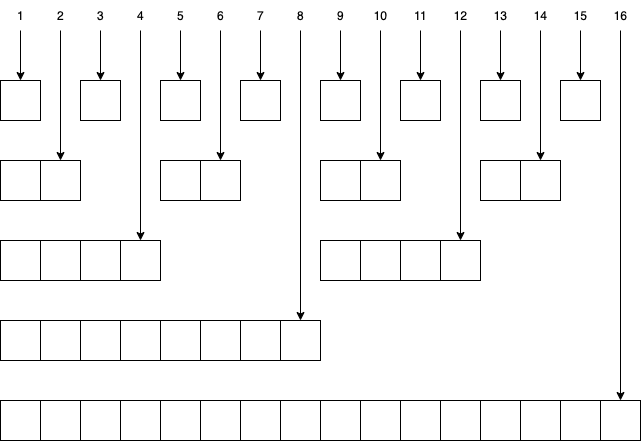
\includegraphics[width=\textwidth]{./Pictures/Pic1.png}
Man beachte den Start der Liste beim Index 1 und nicht 0. Für den Pseudocode wurde eine Indexierung von 0 angenommen, da dies näher an den meisten Programmiersprachen ist.
Wenn man dann $f(a_1,\dots,a_i)$ auslesen will, geht man wie folgt vor:\\
\begin{lstlisting}
f(FT, i) {
    res=iniatializeF //Default Value for f with no input
    //& is the binary AND operator
    for (; i >= 0; i = i-LSB(i)) 
        res = f(res, FT[i]);
    return res;
}
\end{lstlisting}
Für das auslesen braucht man einen Standardwert (res), der für $f(\phi)$ den Wert darstellt. Jetzt geht man in die andere Richtung wie beim Einsetzen vor, anstatt das LSB zu addieren, wird dies abgezogen und in jedem Schritt $res=f(res,FT[i]))$ bestimmt. Bei $11$ wäre dies dann $11\rightarrow 11-1=10 \rightarrow 10-2=8 \rightarrow 8-8=0$.










\section{Dynamisch programmierter Algorithmus \cite{dynamisch}}

\subsection{Herleitung}
Die Grundlage dieses Algorithmus ist der Robinson-Schensted Algorithmus, welcher in erster Linie sog. Young-Tableu berechnet. Das sind Darstellungen von Symmetriegruppen. In dem zugrunde liegenden Paper wird hauptsächlich aus dem Algorithmus eine Vereinfachung hergeleitet, welche das HIS Problem löst, jedoch gibt es anschauchlichere Herleitung, die den Algorithmus besser verdeutlicht.\\
Es handelt sich um einen dynamisch programmierten Algorithmus. Diese haben es an sich, oft zu betrachten, ob die Erweiterung einer bestehenden Lösung um ein Element, sich aus der $"$kleineren$"$ Lösung herleiten lässt, d.h. in dem Fall konkret, ob eine HIS einer Folge \an, auf eine HIS einer um 1 größeren Folge \an$a_{n+1}$ folgern lässt. Dabei wird eine Tabelle geführt, welche für einen Eintrag an der Stelle $i$ die HIS der (Teil-)Folge $a_1\dots a_i$ abspeichert, welche auf $a_i$ endet. Wenn man nun das $i+1$-te Element betrachtet, ergeben sich folgende drei Fälle:
\begin{enumerate}
    \item Die HIS der kleineren Folge bleibt die HIS der größeren Folge.
    \item Die HIS der kleineren Folge kann um das neue Element erweitert werden und ist danach die HIS der größeren Folge.
    \item Die HIS endet auf dem neuen Element, ist aber nicht die vorherige HIS erweitert.
\end{enumerate}
Interessant ist hierbei Fall 3, denn dafür müsste man andere mögliche Durchläufe speichern. In der Tabelle muss also mehr als ein Tupel ggf. sein, da aber insgesamt $n$ Elemente betrachtet werden, also nur eine Teilfolge, die auf einem $a_i$ endet, ist die Tabellengröße $n$. 
Mit dieser Anforderung können die drei Fälle erkannt werden, indem man die größte der erweiterbaren Folgen - also das größte Element kleiner dem Neuen, vgl. $prev$ aus Kapitel 2- mit dem Neuen erweitert, und ggf. Folgeelemente gelöscht werden. Da wir Paare als Elemente haben, und wir eine strikte Monotonie in beiden Elementen wollen (impliziert eine Sortierung, welche $prev$ schneller berechnen lässt), müssen wir ggf. größere Elemente in der ersten Koordinate löschen, die in der zweiten kleiner sind. Dazu eine kleine Erklärung:\\ 
\newtheorem{beispiel}{Beispiel}
\\
Man möchte das Element $(s,t)$ aus der Liste mit der neuen Zahl $a_i=:x$ erweitern und kriegt dann $(x,t+x)$. Alle Elemente $(u,v)$ mit $x \leq u$ kommen in der Liste danach. Jedoch kann man nicht beeinflussen, ob $v$ kleiner $t+x$ ist. Nehmen wir solch ein Element im Folgenden an. Wenn jetzt $(u,v)$ mit einem Element $a_j$ erweitert wird, muss $a_j$ größer als $u$ sein, demnach auch größer als $x$. Da aber auch $t+x$ größer als $v$ ist, ist auch $t+x+a_j$ größer als $v+a_j$. Dies gilt für alle Elemente die $u$ erweitern können, dadurch kann man alle $(u,v)$ mit $v$ kleiner $t+x$ löschen. Diese können nicht mehr die HIS werden, da jede Erweiterung von $(u,v)$ auch eine von $(x,t+x)$ darstellt.\\
Ein kleines Beispiel dazu ist die Folge $4,2,3,6$. Die Werte in der Liste sind bis zum Wert 3 $(2,2),(4,4)$ und danach die 3 eingefügt $(2,2),(3,5),(4,4)$. Für die 6 kommen sowohl $(3,5)$ als auch $(4,4)$ in Frage - $(2,2)$ auch, aber das hilft der Illustration nicht. 3 erweitert mit 6 ist größer, als 4 erweitert. Das liegt daran, dass die zweite Koordinate von $(3,5)$ größer als die in $(4,4)$ ist. Die Zahl 6 kann hier jede andere beliebige Zahl $x$ mit $x>4$ sein und die Aussage bleibt bestehen. Somit kann die $(4,4)$ gelöscht werden nachdem $(3,5)$ eingesetzt wurde, denn alles was $(4,4)$ erweitert, erweitert auch $(3,5)$.
\\
Nach diesem Prinzip ist die Listen in beiden Koordinaten streng monoton steigend. Wenn man also jetzt das letzte Element in der Liste herausnimmt, hat man das Element auf welches die HIS endet und die Summe der HIS.
\begin{beispiel}
    Sei $(a_n)=4;3;6;1;7;9;23$. Für das 5-te Element müssen alle Elemente in der Liste angeschaut werden, welche kleiner als $a_5=7$ sind, das sind 4,3,6 und 1. Die Abbildung unten beschreibt den Zustand der Liste bevor das Element $7$ eingefügt wurde und zeigt, wo es eingefügt werden muss und wie sich der neue Wert ergibt. Die Abbildung darunter beschreibt die Änderung, welche sich bei $a_3=4$ statt $6$ ergeben würde.
\end{beispiel}
\begin{center}
	\begin{tabular}{c}
		
		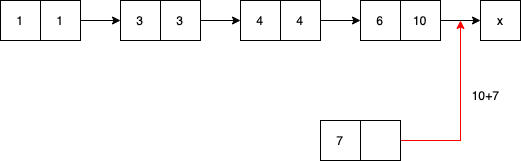
\includegraphics[scale=0.7]{./Pictures/pic2.png}\\
		\hline
		\includegraphics[scale=0.7]{./Pictures/löschen.png}\\
		
	\end{tabular}
\end{center}

\subsection{Algorithmus}
 
Wir wollen also aus der Herleitung der Idee jetzt einen konkreten Algorithmus formulieren. Sei im Folgenden \an eine Folge von natürlichen Zahlen. Als Ordnung und Gewicht nehmen wir die Werte der Zahlen selber. Der Algorithmus läuft dann wie folgt:
\begin{enumerate}
    \item Initialisiere eine leere Liste L und ein leeres Array $nodes$ der Länge $n$.
    \item Gehe nach und nach durch jedes Element $a_x$ in der Folge durch und mache Schritte 3 bis 5.
    \item Finde $(a,b)=prev(L,x)$ und $(c,d)=next(L,x)$.
    \item Solange $(c,d)$ existert und $d<b+x$ ist, führe $delete(L,(c,d))$ aus und setze $(c,d)=next(L,x)$.
    \item Füge $(x,b+x)$ ($(a,b)$ erweitert um x) in die L ein und setze $nodes[x]$ auf $a$.
\end{enumerate}

Das $nodes$-Array kann am Ende zur Rekonstruktion benutzt werden. Es ist auch eine leichte Vereinfachung des originalen Algorithmus vorhanden, da die Gewichtsfunktion hier nur vom Wert der Zahl abhängt und nicht auch noch von der Position. Als Pseudocode wäre das Ganze dann so: \newpage

\begin{lstlisting}[mathescape]
his($a_n$)
{
    %Step 1
    L=$ø$
    %step2
    for(i = 1; i <= n; i++)
    {
        %Step 3
        (s,v)=prev(L,($a_i$,0)) %Finds next smallest Element in List
        (t,w)=next(L,(s,v)) %Finds next largest Element in List

        %Step 4
        while((t,w) != $ø$)
        {
            if(v+$a_i$ < w)
                break;
            delete(L,(t,w))
            (t,w)=next(L,(t,w))
        }

        %Step 5
        if((t,w)$\neq\phi$||$a_i$<t)
       		 insert(L,($a_i$,v+$a_i$))
        nodes[$a_i$]= newnode($a_i$,node[s])
    }
}
\end{lstlisting}
\small Bemerkung:
\begin{quote}
    \footnotesize In Zeile 24 wird $nodes[a_i]$ auf ein $newnode$ Element gesetzt, dies dient zum Speichern der aktuellen Zahl, und an welcher Stelle in $nodes$ die vorherige Zahl in der HIS zu finden ist. Man kann also die HIS in umgekehrter Reihenfolge rekonstruieren. Diese Tabelle ist auch der Grund für das DP, die Liste dient als Hilfe zum Befüllen der Einträge.
\end{quote}
\normalsize


\subsection{Korrektheit}
Für die Korrektheit des Algorithmus' formulieren wir eine Invariante, die nach jeder Iteration des Algorithmus' gelten soll:\\
Sei $L$ die Liste für das Abspeichern der Tupel und $a_1 \dots a_n$ die Folge, für die die HIS gefunden werden soll. Nach der i-ten Iteration für die Zahl $a_i$ gilt: Für jede streng monotone Teilefolge $(b_k)$ in $a_1 \dots a_i$ gibt es ein Tupel $(s,t)$ in der Liste $L$ mit $s\leq b_i$ und $ t \geq \sum_{j=1}^k b_j$. Da für jede endliche Folge eine HIS $b_1 \dots b_k$ existiert, gilt dies auch für die HIS, das heißt, es gibt ein Element $(s,t)$ in L mit $s\leq b_k$ und $t\geq \sum_{j=1}^k b_j$. Wenn man dann aus $L$ das letzte Element (größte) herausnimmt, kriegt man die HIS.

\newtheorem{beweis}{Beweis}

\begin{beweis}
Wir beweisen die Invariante mit Induktion über die aktuelle Iteration im Algorithmus (i-te Iteration). Sei nun $L$ eine Datenstruktur, welche die geforderten Funktionalitäten erfüllt, und $a_1 \dots a_n$ eine Folge an Zahlen (Im Allgemeinen gilt dies auch für eine Menge mit Gewichtung und Ordnung). Für $i=1$ ergibt sich nur eine einzige Teilfolge, nämlich die Folge $a_1$ selber. Nach Zeile 24 im Algorithmus wird bei einem leeren L ein Element in die Liste eingefügt, in dem Fall $(a_i,a_i)$. Daraus folgt die Aussage für $i=1$.\\
Gelte also für ein festes aber beliebiges $i$ die Annahme. Man betrachte nun $a_1 \dots a_{i+1}$ für die $(i+1)$-te Iteration. Nach Annahme gibt für jede monotone Teilfolge $(b_k)$ aus $a_1 \dots a_{i}$ ein Tupel $(s,t)$ in der Liste, welches die Anforderung der Invariante erfüllt. Daraus ergeben sich drei Fälle: $a_{i+1}=b_k$, $a_{i+1}>b_k$ und $a_{i+1} < b_k$. Sei $(s,t)$ das Element aus L, welche für $(b_{k})$ die Invariante erfüllt.
\begin{itemize}
 
    \item $a_{i+1}=b_k$: aus der Monotonie folgt $s\leq a_{i+1}$. Schritt 4 kann also $(s,t)$ nicht entfernen - $(s,t)$ bleibt in der Liste. Entweder ist ein Tupel $(u,v)$ mit $u=a_i$ schon in L oder wird in diesem Schritt eingefügt (Schritt 5). Da nach vorheriger Bemerkung die Liste in beiden Elementen monoton steigend ist, erfüllt $(u,v)$ die geforderte Bedingung.
    \item $a_{i+1}<b_k$: Da nur Elemente nach $prev(L,a_{k+1})$ gelöscht werden, bleibt $(s,t)$ in L und erfüllt damit die Invariante für $(b_k)$.
    \item $a_{i+1} > b_k$: Nach Annahme ist $t$ mindestens so groß wie $\sum_{j=1}^k b_j$. Falls Schritt 4 nicht das Tupel $(s,t)$ löscht, gibt es nichts zu zeigen, da $(a_{i+1},t+a_{i+1})$ für $b_1 \dots b_k a_{i+1}$ die Invariante erfüllt, und $(s,t)$ erhalten bleibt. Falls es gelöscht wird, garantiert Zeile 15, dass das neue Tupel $(a_{i+1},t+a_{i+1})$ die Monotonie von L erfüllt. da $a_{i+1}>b_k$ nach Annahme gilt, ist die Invariante in diesem Fall erfüllt.
\end{itemize}

Aus dem Prinzip der vollständigen Induktion folgt die Aussage für alle $i \in \mathbb{N}$.

\end{beweis}



\subsection{Laufzeitanalyse}
Da für die Erklärung eine Liste verwendet wurde, betrachten wir die Laufzeit im ersten Schritt anhand einer. Da über die Eingabeliste iteriert wird, haben wir in Abhängigkeit dessen Länge $n$ die Schritte 3 bis 5. Schritt 3 führt $prev$ und $next$ aus. In einer Liste benötigt $prev$ im Worst-Case (WC) n Schritte, $next$ ist der Nachfolger, benötigt also nur einen. Schritt 4 betrachtet den Nachfolger von $prev$ aus Schritt 3, diese sind im WC alle bisher eingefügten Elemente. Man muss aber beachten, dass maximal nur n Elemente gelöscht werden können, da wir für jedes Element in $a_1 \dots a_n$ maximal ein Element in die Liste einfügen, d.h. Schritt 4 wird über alle Iterationen gemeinsam maximal n-Mal ausgeführt (Ob Schritt 4 ausgeführt werden muss, benötigt $O(1)$). Hiermit ist die Laufzeit insgesamt im WC $O($Algorithmus ohne Schritt 4$)+n*O($Schritt 4$))$.  Schritt 4 selber ist in linearer Zeit möglich, wenn eine einfach verkette Liste verwendet wird. Schritt 5 ist in konstanter Zeit möglich, da das neue Element nach dem $prev$ aus Schritt 2 kommen muss.
Insgesamt hat man damit für die Liste eine Laufzeit im WC von $O(n^2)+n*O(1)=O(n^2)$\\
Um das ganze auf $O(n$log$(n))$ zu verringern, betrachten wir eine Abwandlung des Algorithmus in einem FT. Die assoziative Funktion ist $max$. Für eine Folge \an, gibt $rang(a_i)$ die Position von $a_i$ in \an ~sortiert an. In einen FT kann ein Wert in $O($log$(n))$ eingefügt werden - die Position ist $rang(a_i)$. Geht man \an ~von $1$ bis $n$ durch, fügt aber bei $rang(a_i)$ ein, hat das zur Folge, dass für Elemente $a_j$ mit $j>i$ aber $rang(a_j)\leq rang(a_i)$ noch kein Wert im FT gespeichert ist, beim Auslesen von $max$ der Einträge $1..rang(a_i)$ den Wert nicht verändern. Genauso gilt auch, dass $max$ nur für Einträge mit $j<i$ und $rang(a_j)\leq rang(a_i)$ den Wert bestimmt. \\
Der Wert im FT an der Stelle $rang(a_i)$ stellt den Wert der HIS  für $a_1 \dots a_i$, welche auf $a_i$ endet. Damit ist auch ohne $next$ und $delete$ durch einen FT gewährleistet, dass in log$(n)$ $prev$ gefunden werden kann. Folgende Abbildung illustriert die Vorgehensweise. Grün bedeutet ein noch nicht geänderter Wert, Blau ein geänderter und Rot der aktuell betrachtete Wert $a_3=6$.\\
\begin{center}
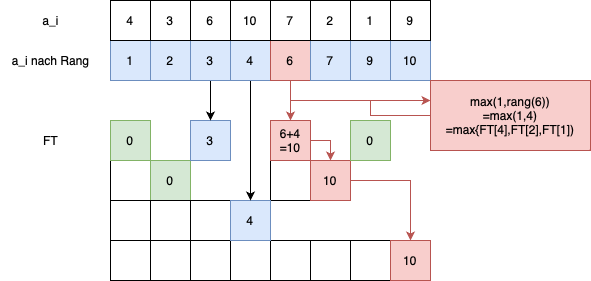
\includegraphics[scale=0.7]{./Pictures/FTexample.png}
\end{center}

Um die HIS zu rekonstruieren, wird ein $nodes$ Array benötigt, welche den neu eingetragenen Wert im FT an der Stelle $i$ (nicht $rang(a_i)$!) abspeichert. Wenn man dann von $n$ bis $1$ ($\sim$ rückwärts) durch $nodes$ läuft und $max(1,n)$ im FT findet, hat man das $a_i$ auf welches die HIS endet. Zieht man dieses vom Wert in $nodes$ ab, erhält man den nächsten Wert, der von der aktuellen Position aus gesucht wird. Durch eine einfache Anpassung, kann man auch bei mehreren Einträgen in $nodes$ mit dem gleichen Wert erkennen, welchen man nehmen muss. Dies sei dem Leser überlassen.

\begin{lstlisting}[mathescape]
res = max(1,FT.length);
for(i=FT.length;i$\geq 0$;i--){
	if(nodes[i]==res){
		print($a_i$);
		res-=$a_i$;
	}
}
\end{lstlisting}



% \section{Sequenzierungsbasierter Algorithmus}
% \subsection{Einführung}
% Der zweite Algorithmus stammt aus dem Bereich der Sequenzierung, genauer der Gensequenzierung. Gurundlage hierfür ist das Problem zwei (wahrscheinlich) ähnliche Genome zu vergleichen. Dafür muss eines der beiden bereits aufgeschlüsselt sein. Man nimmt dafür ähnliche Abschnitte der Genome zusammen, d.h. eine Folge  ist 'ähnlich' zu einer Folge im zweiten Genom (im Originalen Teilfolgen, aber für diese Arbeit reicht es nur Folgen zu betrachten). Alle solche Folgen werden als Paar abgespeichert. Ohne weitere Einschränkung seien die zu vergleichenden Folgen identisch.\\
% Wenn man nun diese Paare als Rechteckte im Raum annimmt (Start- und Endpunkte der Folgen sind jeweils die Ecken) wird nach einer Folge an Rechtecken gesucht, die nicht überlappend sind und der Weg sich immer nach oben rechts bewegt (vgl. Abbildung), dessen Gewichtung am größten ist.

% %Abbildung einfügen

% \subsection{Herleitung}
% Man sieht hier schon zwei parallelen zum HIS Problem. Einererseits ist eine aufsteigende Sequenz gesucht, andererseits haben diese Rechtecke auch eine Gewichtung, denn man möchte so wenig wie möglich aufschlüsseln müssen des zewiten Genoms. Problem ist jedoch die 2-Dimensionalität des Problems. Im folgenden wird eine Abwandlung zum Lösen des Ausgangproblem erklärt, welche die Dimension verringert und mit geschickter Gewichtung und Ordnung das HIS Problem löst. Die Ordnung ist im Folgenden als Priorität bezeichnet.\\
% Als Gewichtung nehmen wir hier die Länge der Folge an, die das Rechteck widerspiegelt. Da die Folgen identisch sind, handelt es sich um Quadrate mit der Länge $s$. Eine direkte Möglichkeit zum finden einer optimalen Folge wäre:\\
% \[
%     g.score=g.weight+max\{f.score | f \ll g\}
% \]

% Dieser Ansatz kann als Grundlage eines Dynamischen Algorithmus dienen, indem man die Quadrate anhand ihrer Startpunkte sortiert. Man sieht recht schnell, dass dies dem Algorithmus aus Kapitel 3 ähnelt in der Idee, denn $f\ll g$ ist vergleichbar mit dem Ansatz, das größte Element zu finden, welches um das Aktuelle erweitert werden kann ($prev$).\\

% \subsubsection*{Optimierung}
% Das ganze kann aber optimiert werden, in dem man sich Eigenschaften der Quadrate im Raum zu Nutze macht. Wenn man die x-Achse von 0 aus nach rechts entlang läuft und sich bei jedem Punkt $a$ anschaut welches die größte bisherige Folge ist, kann man die Quadrate $(s,t)$, die schon abgegangen sind, markieren. Alle diese Quadrate haben $t_1 < a$, die x-Koordinate von $t$ ist kleiner als $a$. $s$ ist also in der Berechnung nicht relevant und damit ist eine Dimension weniger nötig für die Berechnung. \\ Wir betrachten also die y-Koordinaten der Endpunkte aller Quadrate. Nehmen wir nun $(p,v)$ als Koordinaten an, p ist die Priorität (Die Position in der Ausgangsliste) und v ist die y-Koordinate des Endpunkts welche in dem Fall auch die Gewichtung widerspiegelt. Mit diesen Koordinaten bauen wir einen abgewandelten PST auf. Wie genau dieser erstellt wird, ist im Kapitel zur Implementierung beschrieben, wichtig ist aber folgende Eigenschaft hier: Die Blätter sind die Koordinaten. Von links nach rechts gelesen ist es wie in der gegeben Reihenfolge, d.h. das i-linkste Blatt ist das i-te Element $(i,v_i)$. Die inneren Knoten haben eine Priorität von $-\infty$ zu beginn (das ändert sich im Verlauf des Algorithmus') und dienen zum schnelleren finden folgendem Elementes: In einem Bereich von $(0,q)$ soll der Knoten gefunden werden, welcher den größten Score (Größte Summe an Gewichtungen) hat. Dies wird als $RMaxQ(0,q)$ bezeichnet. Da dies ein Blatt sein muss werden in den inneren Knoten diese geschickt gespeichert um schneller an dieses zu gelangen.\\
% An einem inneren Knoten $q$ ist $q.L$ bzw. $q.R$ der linke (rechte) Teilbaum. $q.Cv$ ist die Menge aller Blätter unter $q$ und $q.Pv$ ist das Blatt mit dem größten Score welches nicht in einem Knoten unter $q$ als $Pv$ gespeichert ist (vgl. Abbildung). $q.Hv$ ist das Schwerste Element aus $Cv$.


% \subsubsection*{Berechnung}
% Wenn man jetzt die optimale Folge an Rechtecken will, benötigen wir eine Möglichkeit das Quadrat kleiner dem Punkt $a$ zu finden, welchen den größten Wert hat. Im PST wird dies mit $RmaxQ(0,a)$ gemacht. Genauer wird darauf in Kapitel 6 eingegangen. Wenn dieser Wert gefunden wurde, muss nur noch das Quadrat an der Stelle $a$ angepasst werden um den neuen Wert. Dies wird gemacht in dem der Score geändert und dann ein Durchlauf durch alle Knoten gemacht wird. Dieser Vorgang entspricht dem Einfügen eines neuen Elementes in einer PQ, es wird aber kein Element direkt eingefügt, sondern ein Wert angepasst und dann die Integrität der Datenstruktur widerhergestellt. Auch werden nicht direkt Elemente getauscht, sondern nur die Werte in den Elementen. Dabei wird der abzugehende Teilbaum anhand von $a<h_{v.L}$ bestimmt.

% \subsection{Anpassen an das HIS}
% Wir haben also eine Liste an \an. Als priority nehmen wir die Position der Zahl und als key value den Wert der Zahl. Damit kann dann ein PST aufgestellt werden, welcher nach einem durchlauf von der Liste den Wert der HIS in sich hat am größten Blatt. Ein vereinfachter Pseudocode sieht wie folgt aus:

% \begin{lstlisting}[mathescape]
% his($a_n$)
% {
%     //Wurzel des Baumes
%     root =buildPST($a_n$); 
%     for(i = 1;i <= n; i++)
%     {
%         q = RMaxQ(0,$a_i$);
%         if(q.priority = $-\infty$)
%             continue;
%         root.CV[i].score +=q.score;

%         //Pv neu setzen im Baum
%         updatePv();
%     }
% }
% \end{lstlisting}

% Dieser Peusocode wirkt kurz, ist aber in der Implementierung aufwändiger als der erste Algorithmus.




\section{HIS als Sonderfall des Genomvergleichs \cite{ohlebusch}}

Dieses Kapitel führt das Problem des Genomvergleichs ein, ein Problem aus der Bioinformatik. Kern des Problems ist es zwei Genomen ($\sim$ Zeichenketten), in denen gemeinsame $"$ähnliche$"$ Abschnitte bekannt sind, diese gegenüberzustellen und eine größte Zuordnung zu finden, welche die originale Ordnung der Abschnitte beibehält. Wie festgestellt wird, ob die Abschnitte ähnlich sind, ist für den Algorithmus nicht relevant. 

\subsection{Herleitung}
Betrachtet man zwei Genome $G_1=a_1\dots a_n$ und $G_2=b_1\dots b_m$ über einem Alphabet $\Sigma$, sind zwei Abschnitte $A_1$ und $A_2$ lückenlose Bereiche aus $G_1$ und $G_2$, d.h. es existieren $i,j$ mit $1\leq i \leq j \leq n$ und $k,l$ mit $1\leq k \leq l \leq m$, s.d. $A_1 = a_i\dots a_j$ und $A_2 =b_k \dots b_l$. Man kann diese $"$Übereinstimmung$"$ durch ein Rechteck $R_1=((i,j),(k,l))$ charakterisieren. Man erhält dann eine Menge an Rechtecken $R$, welche alle ähnlichen Abschnitte enthält. Zusätzlich gibt es eine Funktion $f:R \mapsto \mathbb{N}$, welche jedem Abschnitt ein Gewicht ($weight$) zuordnet. Gesucht ist die Teilmenge $C \subset R$, für die die Summe aller Gewichte maximal ist. Zusätzlich dürfen zwei Rechtecke $R_x,R_y \in C$ nicht überlappend sein, also $R_x \ll R_y$ oder $R_y \ll R_x$ muss gelten. Zusätzlich wird ein Wert $score$ für jedes Rechteck $R_i$ gespeichert, welches am Ende für die Menge $R'=\{r | r \ll R_i\} \cup \{R_i\}$ die größtmögliche Summe der Gewichte nach vorheriger Anforderung abspeichert. Anschaulich bedeutet das, dass für ein Rechteck alle anderen Rechtecke betrachtet werden, welche nicht überlappend sind. Von denen wird das mit dem größten Score gewählt und mit $R_i$ erweitert.\\
Dies kann man als rekursive Gleichung formulieren:
\[ R_i.score =  R_i.weight + max\{r.score | r \ll R_i\}\]

\newtheorem{bemerkung}{Bemerkung}
\begin{bemerkung}[Parallele zum ersten Algorithmus]
Schon hier ist die Parallele zum ersten Algorithmus ersichtlich, $max\{r.score | r \ll R_i\}$ ist übertragbar auf $prev$ aus Kapitel 3. Genauso ist hier auch erkennbar, dass man für eine Menge an Rechtecken $R$ mit den Elementen $R_1 \dots R_n$ die obige Gleichung nur Anwenden kann, wenn\\ $max\{r.score | r\ll R_i\}$ bekannst ist, d.h. konkret, dass man für alle $r \ll R_i$ schon den $score$ berechnet haben muss. Also hat der $\ll$-Operator inherent eine Ordnung, nach welcher die Berechnung erfolgen muss. 
\end{bemerkung}


\subsection{erste Formulierung eines Algorithmus'}

\begin{definition}[$RMaxQ$ als Äquivalent zu $prev$] $prev(L,i)$ gibt, falls existent, das größtmögliche Element $y\in L$ zurück, mit $y\leq x$. Dies erweitern wir, indem wir in einem bestimmten Bereich $[a,b]$ das Rechteck mit dem größten $score$ haben wollen. Das bezeichnen wir als $RMaxQ(a,b)$. Im Falle $a=0$ bedeutet dies den Ursprung $(0,0)$.
\end{definition}

Anhand dieser Definition formulieren wir folgende Aussage:
Seien $G_1$ und $G_2$ Genome, $R_1, \dots, R_n$ ähnliche Abschnitte. Für ein $R_i=(s_i,t_i)$ mit $R_j=RMaxQ(0,s_i -(1,1))$ gilt $R_i.score=R_i.weight+R_j.score$. Das bedeutet, dass das Rechteck, welches $RMaxQ(0,s_i-(1,1))$ zurückgibt, auch $max\{r.score | r << R_i\}$ entspricht. Dies gilt per Definition von $RMaxQ(a,b)$,  da für $RMaxQ(0,s_i-(1,1))$ alle Rechtecke angeschaut werden, die vor $R_i$ kommen. Ein erster Algorithmus für das Problem sortiert $R_1,\dots ,R_n$ nach der $x_1$ Koordinate im Start- und Endpunkt und findet anhand dieser Ordnung $RMaxQ(0,R_i-(1,1));$
\begin{lstlisting}[mathescape]
GenomeAlignment(R){
    R=R.sort; //Sort w.r.t. $x_1$ coordinate
    for(i=1;i\leq n; i++){
        $R_j$=RMaxQ(0,$R_i$.s - (1,1));
        $R_i$.score=$R_i$.weight+$R_j$.score;
    }
    return RMaxQ(0,$R_n$.t);
}
\end{lstlisting}

\begin{bemerkung}[kleine Vereinfachung von $RMaxQ$]
Für diesen Algorithmus braucht man sowohl x- und y-Koordinate der Rechtecke, also zwei Werte. Durch die vorhin beschriebene Ordnung von $R_1 \ll \dots \ll R_n$, kann man das ganze verringern. Wir betrachten für $s_i=(x_i,y_i)$ (Den Startpunkt von $R_i$) die x-Koordinate $x_i$. Für diese gilt $x_1 < \dots < x_n$. Betrachten wir nun in der $i$-ten Iteration von $GenomeAlignment$ die Mengen $A=\{R_1,\dots , R_{i-1}\}$ und $I=\{R_i,\dots , R_n\}$. $A$ sind die schon betrachteten Rechtecke, und $I$ welche noch folgen. $RmaxQ(0,s_i-(1,1))$ schaut nur die Rechtecke in $A$ an. Zusätzlich gilt für alle $a \in A: a.s:=(x,y): x < x_i $. Die Startpunkte von allen Rechtecken in $A$ sind links vom Startpunkt von $R_i$. Somit ist die x-Koordinate der Startpunkte nicht mehr relevant, es reicht also eine alternative Definition $RMaxQ'(a,b)$ welche nur Zahlen keine Tupel bekommt, explizit hier $RMaxQ'(0,y_i-1)$.
\end{bemerkung}


\subsection{Anwendung auf den HIS}
Ein noch nicht betrachteter Sonderfall ist, wenn Start- und Endpunkt zusammenfallen, also für ein Rechteck $r=(s,t), s=t$ gilt. In diesem Fall sind die Rechtecke einzelne Punkte in der Ebene. Nun kann man für eine Folge \an ~die Folge an Paaren $(1,a_1),(2,a_2),\dots,(n,a_n)$~in der Ebene betrachten. Für $(i,a_i)$ ist $weight=a_i$.
\begin{center}
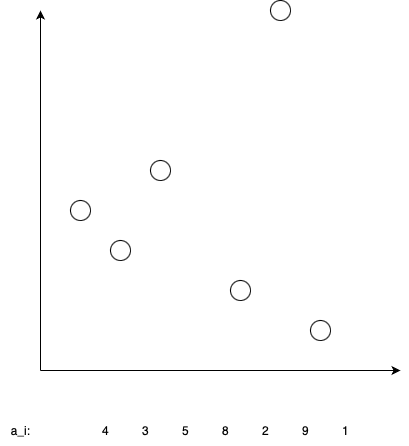
\includegraphics[scale=0.6]{./Pictures/HISGen.png}
\end{center}
\begin{bemerkung}[$RMaxQ(a,b)$ vs. $prev$]
$RMaxQ2(a,b)$ kann ein Rechteck mit Endpunkt $(\_,b)$ bestimmen (wie vorhin angemerkt, ist die x-Koordinate nicht relevant). Deshalb ist es nötig $RMaxQ(0,b-1)$ zu benutzen, $RMaxQ2(0,b)$ kann das Rechteck mit Endpunkt $(\_,b)$ zurückgeben, was offensichtlich nicht gewollt ist. Das bedeutet, dass $RMaxQ(0,b-1)$ äquivalent zu $prev(L,(\_,b))$ ist.  Da wir immer von $0$ ausgehen und nur schon betrachtete Werte in D sind, schreiben wir kurz $RMaxQ2(b)$.
\end{bemerkung}
Folgende Anpassung kann vorgenommen werden, um den Algorithmen an Punkte statt Rechtecke anzupassen:
\begin{lstlisting}[mathescape]
HIS($(a_n)$){
    L = (a_n).map(a_i -> (a_i,0); //Mapping a_i to (weight,score)
    A = new D; //initialising Data Structure D
    for(int i = 1; i \leq n ; i++){
       	q = RMaxQ2(a_i-1);
       	Prec[i] = q.i;
       	a_i.score=a_i.weight+q.score;
       	if(a_i.score > RMaxQ2(a_i).score)
       		insert(a_i);
       		while(a_i.score > next(a_i).score)
       			delete(next(a_i));
    }
}
\end{lstlisting}
\begin{small}
    Bemerkung: $next$ ist wie im Kapitel 2 zu verstehen.
\end{small}

Zum Rekonstruieren wird $Prec$ an der stelle $RMaxQ2(\infty).i$ durchgelaufen. Dies ist identisch zum Vorgehen aus Kapitel 3. Das folgende Unterkapitel beschäftigt sich mit der Frage, was die Unterschiede zwischen den Algorithmen sind und warum ein experimenteller Vergleich keine Aussagekraft über die Entscheidung hat, welcher Algorithmus besser in der Praxis ist.

\subsection{Vergleich}
Beide Algorithmen gehen nach dem gleichen Prinzip vor - das größte Erweiterbare Element zu finden, und dann erweitert einzusetzen. $prev$ und $RMaxQ$ sind in der Funktionsweise also äquivalent - unabhängig von der Datenstruktur. Genauso verwalten beide Algorithmen ein Array für die Rekonstruktion und löschen Elemente, die größer als $prev$ sind, aber im $score$ kleiner als das Neue. Der einzige fassbare Unterschied ist die Reihenfolge, also ob zuerst eingefügt, dann gelöscht wird, oder andersrum. Im Original vom Kapitel $4$ wird zusätzlich ein $(0,0)$ und $(\infty,\infty)$ eingefügt, damit nicht auf $\phi$ überprüft werden muss. Das ist aber eine Frage der Implementierung bzw. Programmierstil, und nicht des Algorithmus'.\\
$"$Note that the Algorithm 8.4 maintains the following invariant: If $q1 < q2 < ··· < ql$ are the entries in the data structure D, then $q1.score \leq q2.score \leq ··· \leq ql.score$.$"$\cite{ohlebusch}- dies beschreibt die Ordnung der Elemente in D. Interessanterweise können aber keine zwei Elemente mit gleichem $score$ in $D$ sein nach Zeile $8$ und $10$. Für den DP Algorithmus gilt $"$We maintain the invariant that L is strictly increasing in both coordinates. Therefore, the ordering based on their first coordinate (the alphabet ordering) can be used to order L. Figure 2 shows the HIS algorithm.$"$\cite{schensted1961longest}. Also auch eine strenge Monotonie der Elemente. Das bedeutet, dass die gleichen Elemente eingefügt und gelöscht werden müssen in einer Iteration, damit die Anforderungen erfüllt bleiben. Einzig in der Frage wie man mit einen Element, welches eingefügt werden soll, umgehen soll, dessen $score$ schon in $D$ Liste, unterscheiden sich die Algorithmen. Der DP Algorithmus löscht so ein Element und fügt das neue ein, dieser Algorithmus verändert D nicht. Wenn man im DP Algorithmus Zeile 15 in $if(v+a_i)\leq w$ umwandelt und in Zeile $16$ ein $continue$ statt $break$ hat, ergibt sich das gleiche Prinzip. Beide Algorithmen unterscheiden sich also minimal in der Vorgehensweise.\\
Da nach dem Gesetz der großen Zahlen es zufällig ist, wie der $score$ für ein Element aussieht, ist der Nutzen direkt abhängig davon, wie viele Elemente mit gleichem $score$ eingefügt werden. Man kann aber wie den DP Algorithmus auch diesen mit einem FT und kriegt dann einen abgewandelten Quellcode, der identisch dem vom DP Algorithmus ist. Die Laufzeitanalyse und Korrektheit ist nahezu identisch aus Kapitel 3 zu übernehmen.





 

\section{Implementierung und Beurteilung}
Die Implementierung findet vollständig in Java statt. Generelle Java Syntax wird nicht erklärt, Besonderheiten wie Interfaces und der '?' Ausdruck werden an der Entsprechenden Stelle erklärt. In Java ist der ø Parameter gleich dem $null$-Verweis. Die Benutzung von Generics kann  \href{https://docs.oracle.com/javase/tutorial/java/generics/index.html}{in\cite{oracle}} nachgelesen werden. Die Liste wird referenzbasiert implementiert, um Aufrückoperationen in einem Array zu vermeiden. 
\subsection{Datenstrukturen}
\subsubsection{sortierte Liste (sorted linked list)}
\normalsize
Wie im Kapitel 3 besprochen, benötigen wir eine Datenstruktur, welche Elemente mit einer Ordnung abspeichern kann. Dafür gibt es in den meisten Programmiersprachen ein $Array$, eine Datenstruktur mit fester Länge und konstanter Zugriffszeit. Auf dieser kann man eine Ordnung definieren. Problem bei  einem Array ist, dass nicht alle Plätze benötigt werden zu jeder Zeit, und, dass das Einfügen zwischen zwei Elementen einen höheren Aufwand hat (WC ist $O(n)$). Der Grund dafür ist das Aufschieben aller nachfolgenden Elemente nach dem eingefügten Element. Damit ergibt sich auch für das Array für den Algorithmus eine Laufzeit von $O(n^2)$\\
Beide Probleme werden bei einer (einfach) verketten Liste gelöst. Anstatt eine feste Größe festzulegen, definiert man ein Startelement (zusätzlich eine Methode die das Startelement verändern kann) und gibt bei jedem Element an, welches als nächstes kommen soll. Das letzte Element verweist dann auf ø.\\

%Illustration dazu einfügen

Jedoch ist die Zugriffszeit hierbei ein Problem, da man Element für Element durchgehen muss, bis das gewünschte Element gefunden ist (WC $O(n)$). Um der Idee einer Liste aus Kapitel 2 näher zu kommen, wird auf eine Implementierung mit Array verzichtet.

\subsubsection*{Tupel}
Ein Tupel ist ein simples Objekt welches zwei vergleichbare Variablen beinhaltet. Die $compareTo$ Methode gibt den Vergleich der ersten Koordinate von zwei Tupeln zurück, falls diese aber die gleiche Gewichtung haben, wird der Vergleich der zweiten Koordinate zurückgegeben. Das ist eine sehr allgemeine Formulierung ($\sim$Generics), aber konkret betrachten wir Paare an natürlichen Zahlen, bei denen $(a,b)<(x,y)$ bedeutet, dass $a<b \vee (a\geq b \wedge x<y)$ gilt. \newpage

\begin{lstlisting}[mathescape]
class Tuple<T extends Comparable<T>> implements DualArgument<Tuple<T>>{
    T first;
    T second;

    public Tuple(T first, T second){
        this.first=first;
        this.second=second;
    }

    @Override
    public int compareTo(Tuple<T> o) {
        if(first.compareTo(o.first)!=0)
            return first.compareTo(o.first);
        else
            return second.compareTo(o.second);
    }
}
 \end{lstlisting}
 
\textbf{Bemerkung}: Zeile 1: DualArgument ist ein kleines Interface, welches den Datentypen T dazu zwingt eine Methode zu haben, die nur das zweite Element in zwei Tupeln vergleicht. Comparable wird hier für T festgelegt, da $first$ und $second$ jeweils nur einen Wert darstellen.

\subsubsection*{Element}
Ein Element ist ein Objekt, welches ein Tupel von zwei natürlichen Zahlen beinhaltet. Außerdem gibt es eine Variable welche auf das nächste Element verweist. Als Methoden gibt es eine zum Setzen des Folgelementes und eine die ein Tupel in einem anderen Element in der zweiten Koordinate vergleicht.\newpage

\begin{lstlisting}[mathescape]
class Element<T extends DualArgument<T>> implements DualArgument<Element<T>> {
    T content;
    Element<T> next;

    public Element(T content){
        this.content=content;
        next=null;
    }

    public void setNext(T next){
        this.next=new Element<T>(next);
    }

    @Override
    public int compareTo(Element<T> o) {
        return content.compareTo(o.content);
    }

    @Override
    public int compareToSecond(Element<T> o) {
        return content.compareToSecond(o.content);
    }
}
\end{lstlisting}




%Erklärung einfügen

 

\subsubsection*{Liste}
Die Liste ist ein etwas größerer Block, weswegen nach und nach die Methoden angegeben werden. Eine Liste speichert Zugriffe auf Head und Tail (Tail braucht man ggf. nicht speichern). Eine vollständige Implementierung ist im Anhang beigelegt.

\begin{lstlisting}[mathescape]
public class LinkedList<T extends DualArgument<T>> {
    Element<T> head; //First Element 
    Element<T> tail; //Last Element
    
}
\end{lstlisting}
Beim Einfügen eines neuen Elementes $q$ werden zwei Elemente $s,v$ gefunden mit $s\leq q \leq v$. $s$ kriegt als Nachfolger $q$ und $q$ als Nachfolger $v$. Hier gibt es ein paar Sonderfälle. Bei einer leeren Liste wird Head und Tail auf das Neue gesetzt. Wenn das neue Element der neue Head wird, dann gibt es kein vorheriges Element, aber der Head muss neu gesetzt werden. Für Tail gilt das gleiche, bloß dass es keinen Nachfolger für das Neue gibt. Falls es nur ein Element in der Liste gibt, wird geprüft, ob das Neue davor oder danach kommt.\\
Die Stelle, an der es eingefügt werden muss, wird durch den Vergleich zweier aufeinanderfolgenden Elementen in der Liste gefunden. Wenn das neue Element zwischen den Beiden gehört, ist die Stelle gefunden. Hierdurch ergeben sich mehere Vergleiche auf den ø (null) Parameter.

\begin{lstlisting}[mathescape]
public void insert(T toInsert) {
        Element<T> newElement = new Element<T>(toInsert);
        if (head == null) {  //no element in the list
            head = newElement;
            tail = head;
        } else if (head.equals(tail)) {
            if (head.compareTo(newElement) < 0) {
                head.next = newElement;
                tail = newElement;
            } else {
                newElement.next = head;
                head = newElement;
            }
        } else if (head.compareTo(newElement) > 0) {
            newElement.next = head;
            head = newElement;
        } else {
            //Now we have at least two Elements in the list
            Element<T> current = head;
            
            /*We check whether the newElement should go in between 
            the current and its successor
            current.next!=null assures we can compare it to the 
            next Element, if not we now are at the tail*/
            
            while (current.next != null &&
                current.next.compareTo(newElement) < 0) {
                if (current.next.compareTo(newElement) == 0)
                    break;
                current = current.next;
            }
            if (current.equals(tail)) {
                tail = newElement;
            }
        newElement.next = current.next;
        current.next = newElement;

    }
}
\end{lstlisting}

Die letzte Funktionalität von Bedeutung ist die $prev$ Methode aus kapitel 2. $next$ wird nicht benötigt, denn dies ist der nachfolger von $prev$, oder falls dieser nicht Existiert, der Head der Liste. Dabei geht die Methode sehr ähnlich wie das Einfügen vor und findet die Stelle zwischen der die neue Zahl in die Liste reingehört und gibt das kleinere Element zurück. Ähnliche Sonderfälle wie beim Einfügen werden auch behandelt.


\begin{lstlisting}[mathescape]
public Element<T> prev(Element<T> compareTo) {
        Element<T> current = head;
        if (current == null)
            return null;
            
        if (current.compareTo(compareTo) > 0)
            return null;
            
        if (current.equals(tail)) {
            return current.compareTo(compareTo) < 0 ?
                current : null;
        }
        
        //Now we have at least two Element in the list
        Element<T> next = current.next;
        while (next != null &&
        next.compareTo(compareTo) < 0) {
            current = next;
            next = next.next;
        }
        return current;
    }
\end{lstlisting}
\begin{small}
    \footnotesize Zeile 8: der '?' Ausdruck prüft die Anweisung davor auf $true$ oder $false$ und gibt bei $true$ das vor dem : zurück, bei $false$ das danach.\\ Zusätzlich ist eine Implementierung unter Benutzung der Java Standard-Bibliothek (v.a. der ArrayList) im Anhang beigelegt. Diese hat sich im Vergleich zu meiner Objekt-basierten als gleichgültig rausgestellt. Unterschiede in der Laufzeit waren weniger als $5\%$ bei mehr als 1000 Durchläufen mit zufälliger Eingabe. Dabei ist der Unterschied wsl. auf die Inkonsistenz der Zeitmessung in Java zurückzuführen, da sowohl meine Implementierung als auch die Standard schneller war für verschiedene Eingaben.
\end{small}

\subsubsection*{newNodes}
newNodes ist einer Liste ähnlich , welche nicht auf eine Ordnung überprüfen muss, da die Reihenfolge hier eine Rolle spielt. Eine kleine Methode zur Rekonstruktion ist beigefügt. Die Berechnung der HIS kann genauso gemacht werden in dem man als Zahlen und nicht als String arbeitet.

\begin{lstlisting}[mathescape]
class newNode{
    int current;
    newNode next;

    public newNode(int current, newNode next){
        this.current=current;
        this.next=next;
    }

    public String evalString(){
        String output=current+" ";
        if(next==null) return output;
        else
            return next.evalString() + output;
    }
}
\end{lstlisting}

\subsubsection{Fenwick Tree (FT) \cite{fenwick}}
Ein FT ist für eine Liste an Eingaben $a_i \dots a_n$ als ein Array implementiert, ähnlich wie man Priority Queues als Array darstellen kann. Die beiden Operationen $insert$ und $max$ sind direkt übertragbar in Java. Da es keine Methode für das Bestimmen vom LSB(i) gibt, ist dies mit den binären Operatoren $|=$ und $\&=$ implementiert. Auch muss man es leicht anpassen, da Arrays in Java beim Index 0 beginnen, und nicht bei $1$. Man kann um das zu umgehen, ein Array der Größe $n+1$ erstellen.
\subsubsection*{$insert(D,i,v)$}
\begin{lstlisting}
public static void set(int[] t, int i, int value) {
        for (; i < t.length; i |= i + 1)
            t[i] = Math.max(t[i], value);
}
\end{lstlisting}

\subsubsection*{$max(a_1,\dots,a_i)$}
\begin{lstlisting}
public static int max(int[] t, int i) {
        int res = Integer.MIN_VALUE;
        for (; i >= 0; i = (i & (i + 1)) - 1)
            res = Math.max(res, t[i]);
        return res;
}
\end{lstlisting}

\newpage


\subsection{Programmierung}
Für den dynamischen Algorithmus  kann die Implementierung sehr nah an dem Pseudo-Code stattfinden. Hierbei ist node der Rückgabewert der Methode für die Rekonstruktion der HIS und die Eingabe ist ein Array an Integers
\begin{lstlisting}[mathescape,language=Java]
public static newNode HIS(int[] a) throws Exception {
    //step 1
    newNode[] nodes=new newNode[Arrays.stream(a).max().getAsInt()+1];
    LinkedList<Tuple<Integer>> L =
        new LinkedList<Tuple<Integer>>();
    //step 2
    for(int i = 0; i < a.length;i++){
        //step 3
        Element<Tuple<Integer>> compareTo = 
            new Element<>(new Tuple<Integer>(a[i], 0));
        Element<Tuple<Integer>> prev = L.prev(compareTo);
        Tuple<Integer> sv = prev!=null ? 
            prev.content : new Tuple<Integer>(0,0);
        Element<Tuple<Integer>> next= 
        (sv.equals(new Tuple<>(0,0))) ?
            null : prev.next;
        //step 4
        if(L.head!=null&&L.head.compareTo(compareTo)>=0)
            next=L.head;
        while(next != null){
            Tuple<Integer> tw = next.content;
            if(sv.second+a[i]<tw.second){
                break;
            }
            L.delete(next);
            next=next.next;
        }
        //step 5
        L.insert(new Tuple<Integer>(a[i],sv.second+a[i]));
        nodes[a[i]] = new newNode(a[i],nodes[sv.first]);
    }
    newNode node = nodes[L.getTail().content.first];
    return node;
}
\end{lstlisting}

Der zweite Algorithmus im FT funktioniert etwas abgewandelt nach dem gleichem Prinzip. Für $a_1\dots a_n$ bezeichnet $rank(a_i)$ den Rang des Elementes in der Liste, d.h. welche Position $a_i$ in der List nach einem Sortiervorgang hat. Nach diesem Rang werden die Elemente in dem FT eingefügt mit der Max-Operation. Hat ein Element $a_i$ Rang $r$ wird es an der Stelle $r$ eingefügt nach der Operation. Wenn ein Wert noch nicht belegt ist, wird es mit 0 initialisiert. Falls man auch negative Werte für $a_i$ zulässt, muss es mit dem kleinst möglichem Wert initialisiert werden. \\
Die Werte werden der Position nach eingefügt, aber der Index ist der Rang in $a$, d.h. Einträge mit Index $j<i$ im FT für die Elemente $x,y$ mit $rank(x)=j,rank(y)=i$ ist 0, g.d.w. $index(x)>index(y)$, d.h. das kleinere Element kommt nach dem größeren Element in der Liste $a$. Damit ist gewährleistet, dass das Maximum von den bisherigen Elementen $a_j$ gefunden wird mit $index(a_j)<index(a_i)$. Ein Algorithmus zum finden des Ranges eines Elementes ist in\cite{rank}  für Java zu finden. Das Prinzip vom ersten Algorithmus angewandt, bedeutet, dass Schritt 4 und die Bedingung in Schritt 5 komplett entfallen. Warum das so ist, kann in\cite{wordpress} nachgelesen werden.
\begin{lstlisting}
static int HIS(int[] test){
       int[] rank = findRank(test);
       int[] maxbit = new int[test.length];
       int[] nodes = new int[test.length];
       for(int i =0; i< test.length;i++){
           int r = rank[i];
           int s = max(maxbit,r);
           set(maxbit,r,test[i]+s);
           nodes[i]=test[i]+s;
       }
       /*int max =max(maxbit,test.length-1);
        for(int i = test.length-1; i >=0;i--){
            if(nodes[i]==max){
                System.out.println(test[i]);
                max-=test[i];
            }
        }*/
       return max(maxbit,test.length-1);
}
\end{lstlisting}
Der kommentierte Bereich dient der Rekonstruktion der HIS mit dem Array $nodes$, welches an der Stelle $i$, den Wert der $heaviest$ $subsequence$ von $a_1 \dots a_i$ hat die auf $a_i$ endet. 



\subsection{Laufzeitenvergleich}

Auf einen Apple MacBook M1 ergeben sich folgende Zeiten: Bei einer Eingabe von $10^7$ Elementen hat die Implementierung mit einer Liste nach einer halben Stunde noch kein Ergebniss geliefert, bei der Implementierung mit FT ergab sich eine Zeit von ca. 7 Sekunden. Bei kleineren Längen gab der DP Algorithmus und die Abwandlung aus Kapitel 4 keine nennenswerten Unterschiede, welche in einer langsamen Datenstruktur wie der Liste eigentlich zu erwarten wären, deswegen schließe ich hier, dass beide Algorithmen gleichwertig benutzt werden können. Der Unterschied zwischen Liste und FT ist aber nicht mehr im Promille Bereich, somit ist eine Implementierung mit einem FT immer einer mit verketteter Liste vorzuziehen. Der Grund für diese Laufzeitunterschiede ist die effektive Benutzung der binären Operationen im FT und die langsame Implementierung von $prev$ in einer Liste. Weiter ist die Verwendung von expliziten Referenzen in der Liste ein großer Faktor, der im FT wegfällt. 



\section{Schlussfolgerungen}
Die Ausgangsfrage, welcher Algorithmus besser ist, führt auf die dahinterliegende Datenstruktur zurück, da beide Algorithmen auf die fast gleiche Weise funktionieren. Eine Implementierung mit Liste ist einfacher zu verstehen, jedoch in der Praxis und Theorie langsamer in der Laufzeit als ein FT. Es ergibt sich also eine Implementierung mit FT vorteilhafter als eine Liste.
\section*{Anhang}
Link zum kompletten GitHub-Repository mit dem verwendeten Code:\\ \href{https://github.com/LeoDeMonetize/Bachelorarbeit}{GitHub-Repo} (https://github.com/LeoDeMonetize/Bachelorarbeit)

\newpage
\bibliographystyle{plain}
\bibliography{refs}
\end{document}
